\documentclass{beamer}
\usepackage{tcolorbox}
\usepackage{amsmath}
\usepackage{tikz}
\usepackage{pgfplots}
\usepackage{adjustbox}


%\beamerdefaultoverlayspecification{<+->}
\newcommand{\data}{\mathcal{D}}

\DeclareMathOperator*{\argmin}{arg\,min}

\newcommand\Item[1][]{%
	\ifx\relax#1\relax  \item \else \item[#1] \fi
	\abovedisplayskip=0pt\abovedisplayshortskip=0pt~\vspace*{-\baselineskip}}


\usetheme{metropolis}           % Use metropolis theme


\title{Maths for ML II}
\date{\today}
\author{Nipun Batra}
\institute{IIT Gandhinagar}
\begin{document}
  \maketitle
  
  
  
% \section{Linear Regression}

\begin{frame}{Contour Plot}

 $z = f(x,y) = x^{2} + y^{2}$\\

\begin{columns}
	\pause \begin{column}{0.6\textwidth}
		\begin{adjustbox}{max totalsize={\textwidth},center}
			
		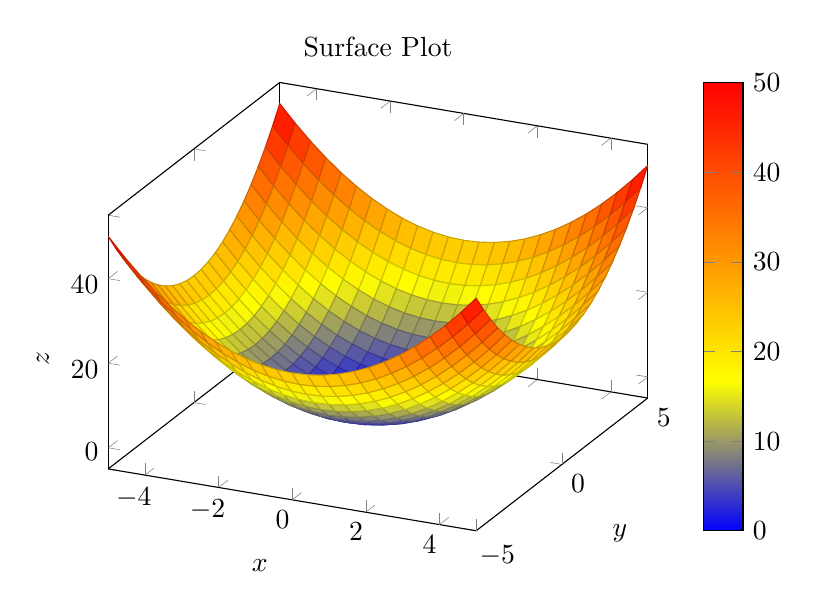
\begin{tikzpicture}
		\begin{axis}[colorbar,xlabel=$x$, ylabel=$y$, zlabel=$z$,title={Surface Plot}]
		\addplot3[
		surf,
		]
		{x^2+y^2};
		\end{axis}
		\end{tikzpicture}
	\end{adjustbox}

	\end{column}
	\pause \begin{column}{0.5\textwidth}
				\begin{adjustbox}{max totalsize={\textwidth},center}
		\begin{tikzpicture}
		\begin{axis}
		[
		title={Contour plot, view from top},
		view={0}{90},
		xlabel=$x$,
		ylabel=$y$,
		axis x line*=bottom,
		axis y line*=left,
		xtick align=outside,
		ytick align=outside,
		unit vector ratio*=1 1 1,
		]
		\addplot3[
		contour gnuplot={number=14,}
		]
		{x^2+y^2};
		\end{axis}
		\end{tikzpicture}
		\end{adjustbox}
	\end{column}
\end{columns}
 
 Then plot $f(x,y)=K$ for varying K.

 
\end{frame}


\begin{frame}{Contour Plot}

$z = f(x,y) = x^{2}$\\

\begin{columns}
	\pause \begin{column}{0.6\textwidth}
		\begin{adjustbox}{max totalsize={\textwidth},center}
			
			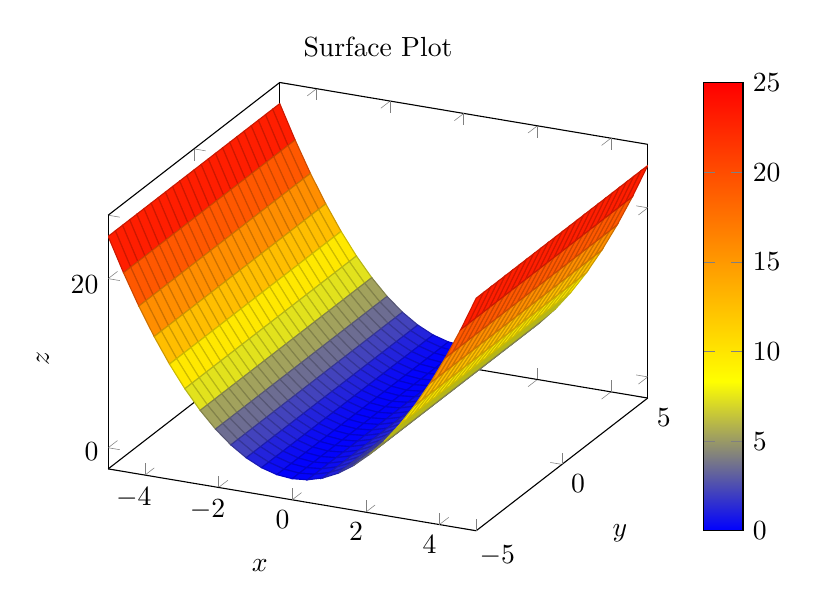
\begin{tikzpicture}
			\begin{axis}[colorbar,xlabel=$x$, ylabel=$y$, zlabel=$z$,title={Surface Plot}]
			\addplot3[
			surf,
			]
			{x^2};
			\end{axis}
			\end{tikzpicture}
		\end{adjustbox}
		
	\end{column}
	\pause \begin{column}{0.5\textwidth}
		\begin{adjustbox}{max totalsize={\textwidth},center}
			\begin{tikzpicture}
			\begin{axis}
			[
			title={Contour plot, view from top},
			view={0}{90},
			xlabel=$x$,
			ylabel=$y$,
			axis x line*=bottom,
			axis y line*=left,
			xtick align=outside,
			ytick align=outside,
			unit vector ratio*=1 1 1,
			]
			\addplot3[
			contour gnuplot={number=14,}
			]
			{x^2};
			\end{axis}
			\end{tikzpicture}
		\end{adjustbox}
	\end{column}
\end{columns}

Then plot $f(x,y)=K$ for varying K.


\end{frame}

\begin{frame}{Contour Plot}

$z = f(x,y) = |x|+|y|$\\

\begin{columns}
	\pause \begin{column}{0.6\textwidth}
		\begin{adjustbox}{max totalsize={\textwidth},center}
			
			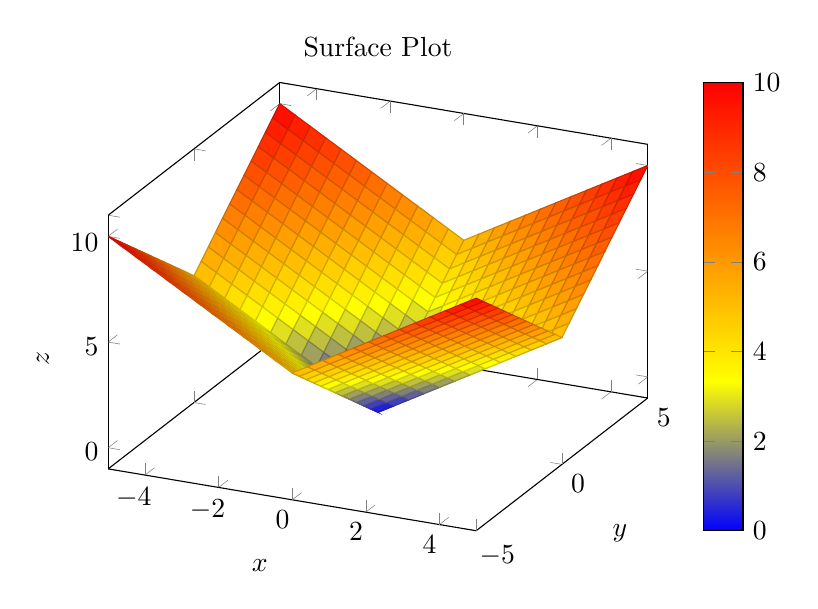
\begin{tikzpicture}
			\begin{axis}[colorbar,xlabel=$x$, ylabel=$y$, zlabel=$z$,title={Surface Plot}]
			\addplot3[
			surf,
			]
			{abs(x)+abs(y)};
			\end{axis}
			\end{tikzpicture}
		\end{adjustbox}
		
	\end{column}
	\pause \begin{column}{0.5\textwidth}
		\begin{adjustbox}{max totalsize={\textwidth},center}
			\begin{tikzpicture}
			\begin{axis}
			[
			title={Contour plot, view from top},
			view={0}{90},
			xlabel=$x$,
			ylabel=$y$,
			axis x line*=bottom,
			axis y line*=left,
			xtick align=outside,
			ytick align=outside,
			unit vector ratio*=1 1 1,
			]
			\addplot3[
			contour gnuplot={number=14,}
			]
			{abs(x)+abs(y)};
			\end{axis}
			\end{tikzpicture}
		\end{adjustbox}
	\end{column}
\end{columns}

Then plot $f(x,y)=K$ for varying K.


\end{frame}

\begin{frame}{Contour Plot}

$z = f(x,y) = (x^2)*y$\\

\begin{columns}
	\pause \begin{column}{0.6\textwidth}
		\begin{adjustbox}{max totalsize={\textwidth},center}
			
			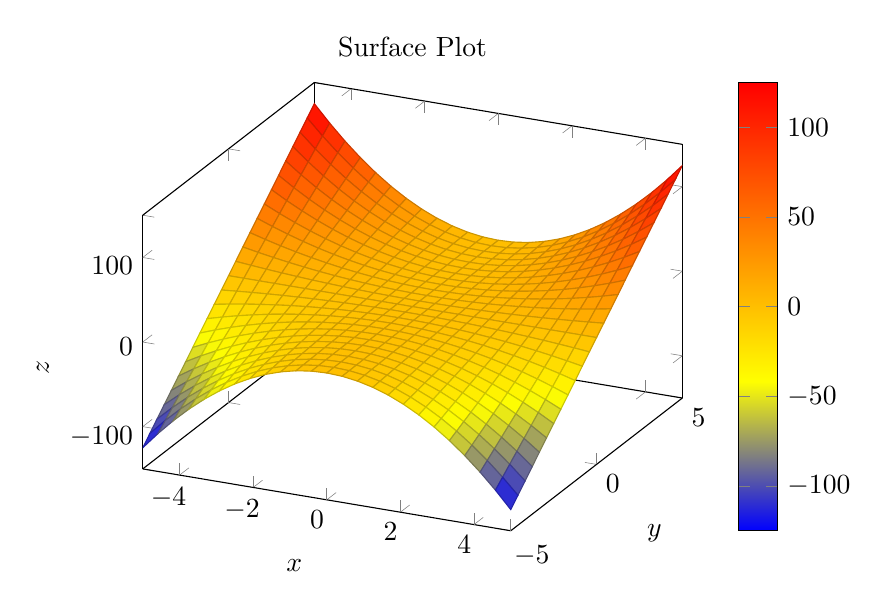
\begin{tikzpicture}
			\begin{axis}[colorbar,xlabel=$x$, ylabel=$y$, zlabel=$z$,title={Surface Plot}]
			\addplot3[
			surf,
			]
			{(x^2)*y};
			\end{axis}
			\end{tikzpicture}
		\end{adjustbox}
		
	\end{column}
	\pause \begin{column}{0.5\textwidth}
		\begin{adjustbox}{max totalsize={\textwidth},center}
			\begin{tikzpicture}
			\begin{axis}
			[
			title={Contour plot, view from top},
			view={0}{90},
			xlabel=$x$,
			ylabel=$y$,
			axis x line*=bottom,
			axis y line*=left,
			xtick align=outside,
			ytick align=outside,
			unit vector ratio*=1 1 1,
			]
			\addplot3[
			contour gnuplot={number=14,}
			]
			{(x^2)*y};
			\end{axis}
			\end{tikzpicture}
		\end{adjustbox}
	\end{column}
\end{columns}

Then plot $f(x,y)=K$ for varying K.


\end{frame}


\begin{frame}{Contour Plot}

$z = f(x,y) = xy$\\

\begin{columns}
	\pause \begin{column}{0.6\textwidth}
		\begin{adjustbox}{max totalsize={\textwidth},center}
			
			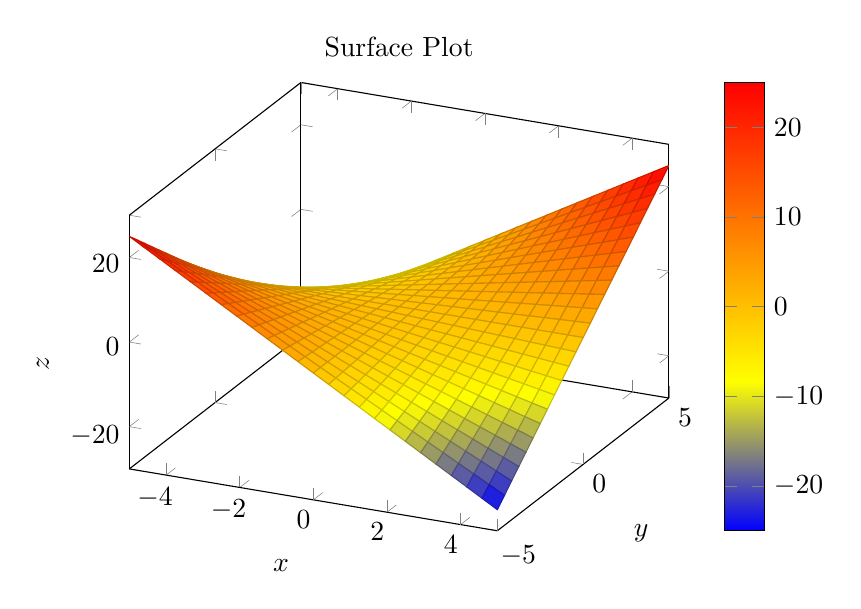
\begin{tikzpicture}
			\begin{axis}[colorbar,xlabel=$x$, ylabel=$y$, zlabel=$z$,title={Surface Plot}]
			\addplot3[
			surf,
			]
			{x*y};
			\end{axis}
			\end{tikzpicture}
		\end{adjustbox}
		
	\end{column}
	\pause \begin{column}{0.5\textwidth}
		\begin{adjustbox}{max totalsize={\textwidth},center}
			\begin{tikzpicture}
			\begin{axis}
			[
			title={Contour plot, view from top},
			view={0}{90},
			xlabel=$x$,
			ylabel=$y$,
			axis x line*=bottom,
			axis y line*=left,
			xtick align=outside,
			ytick align=outside,
			unit vector ratio*=1 1 1,
			]
			\addplot3[
			contour gnuplot={number=14,}
			]
			{x*y};
			\end{axis}
			\end{tikzpicture}
		\end{adjustbox}
	\end{column}
\end{columns}

Then plot $f(x,y)=K$ for varying K.


\end{frame}









\begin{frame}{Contours plots and gradients}
    
    
    Gradient denotes the steepest change.\\
    All points on the contour have the same $f(x,y)$\\
    
    
\end{frame}

\begin{frame}{Contour Plot And Gradients}

$z = f(x,y) = x^{2} + y^{2}$\\

\begin{columns}
	\pause \begin{column}{0.6\textwidth}
		\begin{adjustbox}{max totalsize={\textwidth},center}
			
			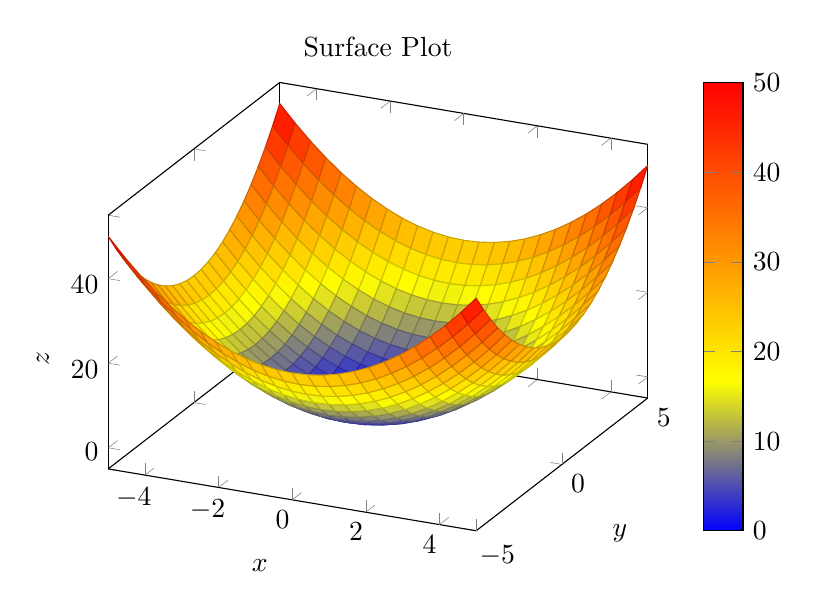
\begin{tikzpicture}
			\begin{axis}[colorbar,xlabel=$x$, ylabel=$y$, zlabel=$z$,title={Surface Plot}]
			\addplot3[
			surf,
			]
			{x^2+y^2};
			\end{axis}
			\end{tikzpicture}
		\end{adjustbox}
		
	\end{column}
	\pause \begin{column}{0.5\textwidth}
		\begin{adjustbox}{max totalsize={\textwidth},center}
			\begin{tikzpicture}
			\begin{axis}
			[
			title={Contour plot, view from top},
			view={0}{90},
			xlabel=$x$,
			ylabel=$y$,
			axis x line*=bottom,
			axis y line*=left,
			xtick align=outside,
			ytick align=outside,
			unit vector ratio*=1 1 1,
			]
			\addplot3[
			contour gnuplot={number=20,}
			]
			{x^2+y^2};
			\addplot3[black,
			quiver={
				u={2*x},
				v={2*y},
				scale arrows=0.1,
			},
			-stealth,samples=10]
			{x^2+y^2};
			\end{axis}
			\end{tikzpicture}
		\end{adjustbox}
	\end{column}
\end{columns}

Then plot $f(x,y)=K$ for varying K.


\end{frame}








\begin{frame}{Contour Plots and Gradients}
    
    Gradient denotes the direction of steepest descent.\\
    All points on the contour have the same f(x,y).\\
    Gradient denotes the direction in which there is a maximum increase in f(x,y)\\

    
    
\end{frame}





\end{document}